\section{NETWORK SERVER CONFIGURATION}

In this case, the Network Server is an instance of \texttt{ResIoT}\cite{ResIOTLoRaWANNetwork}. This instance needs to be configured for each node created.

\subsection{Node configuration}

For this case, the node follows the next configuration and definitions:
\begin{itemize}
    \item \textbf{Type of activation}: In this project, the node uses \acrfullr{otaa}, which gives the possibility of changing the network on startup. 
    This method needs some configuration in the node in the form of some identifiers and an \texttt{APP\_KEY}.The configuration for the device is done in 
    the main module and can be seen in \autoref{fig:nodeconfig}.
    \begin{figure}[H]
        \centering
        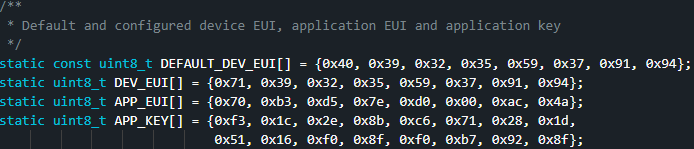
\includegraphics[width=0.85\textwidth]{images/6/Node_config.png}
        \caption{Configuration for the \texttt{OTAA} in the node}
        \label{fig:nodeconfig}
    \end{figure}
    \begin{itemize}
        \item \texttt{DEV\_EUI}: The unique identifier specified by the teachers, in this project, the first byte is $0x71$.
        \item \texttt{APP\_EUI}: The unique identifier for the end application in the network server.
        \item \texttt{APP\_KEY}: This key is used to generate the two keys for the MAC layer and the payload.
    \end{itemize}
    \item \textbf{Type of device}: the node works in class A of \acrshort{lorawan}. It will open 2 specific RX windows after a TX.
\end{itemize}

\subsection{Node definition in the network server}

In the network server, a node was defined with the next characteristics:
\begin{itemize}
    \item \textbf{Name}: \texttt{NODE\_SN\_GROUP\_A}.
    \item \textbf{Node AUTH}: \texttt{LoRaWAN OTAA Class A}.
    \item \textbf{Device EUI}: The same defined in the node configuration in \autoref{fig:nodeconfig}.
    \item \textbf{Application}: The app that shares the same \texttt{APP\_EUI} as in the \autoref{fig:nodeconfig}. In this case, \\ \texttt{RRSS2024\_AppEUI}, that has the configuration of \autoref{fig:appconfig}.
    \begin{figure}[H]
        \centering
        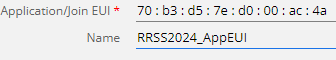
\includegraphics[width=0.6\textwidth]{images/6/AppName.png}
        \caption{App configuration in the network server}
        \label{fig:appconfig}
    \end{figure}
    \item \textbf{APP\_KEY}: The same defined in the node configuration in \autoref{fig:nodeconfig}.
    \item \textbf{LoRaWAN Network Server}: This field points to the server ``eu72.resiot.io\:7677'', configured as a \acrshort{lorawan} Europe server (\texttt{868 MHz}) for Class A+C nodes.
    \item \textbf{Advanced LoRaWAN configuration}: the most important one is that it has \acrfullr{adr}. The reception windows offset are also by default.
    \item \textbf{Node Fields}: These elements allow for dynamic updates of the dashboard. The ones defined and used are as follows:
    \begin{table}[H]
        \begin{center}
            \begin{tabular}{|p{0.20\textwidth} | p{0.20\textwidth} |c| p{0.20\textwidth}| p{0.20\textwidth}|}
                \hline
                \textbf{Field Name} & \textbf{Content Type} & \textbf{Example value} & \textbf{Predefined in the node?}\\
                \hline
                Latitude & Numeric & $40.233921051$ & Yes \\
                \hline
                Longitude & Numeric & $-3.377102145$ & Yes \\
                \hline
                Altitude & Numeric & $665$ & Yes \\
                \hline
                Altitude & Numeric & $665$ & Yes \\
                \hline
                X\_Acc & Numeric & $-0.4692$ & No \\
                \hline
                Y\_Acc & Numeric & $0.0574608$ & No \\
                \hline
                Z\_Acc & Numeric & $9.65342109375$ & No \\
                \hline
                Temperature & Numeric & $23.02$ & No \\
                \hline
                Humidity & Numeric & $54.4$ & No \\
                \hline
                Clear & Numeric & $980$ & No \\
                \hline
                Red & Numeric & $365$ & No \\
                \hline
                Green & Numeric & $383$ & No \\
                \hline
                Blue & Numeric & $346$ & No \\
                \hline
                Light & Numeric & $3.8$ & No \\
                \hline
                Moisture & Numeric & $15.8$ & No \\
                \hline
                LEDStatus & String & OFF & No \\
                \hline
            \end{tabular}
        \end{center}
        \caption{Configuration of the node fields in the ResIoT application.}
        \label{Connections3}
    \end{table}
\end{itemize}

Finally, for the node, 4 commands were defined to control the RGB Led connected to the node.
\begin{itemize}
    \item LED OFF
    \item LED RED
    \item LED GREEN
    \item LED BLUE
\end{itemize}
\subsection{LUA Scripting}
\subsubsection*{On RX}
For the automations of the node in the ResIoT application, a smart scene was defined to run on RX. This scene processes all the messages that the board sends.

The scene in this case is the \texttt{SN\_TEST\_A}, with the hex id $73636531313632$. It is configured with a maximum number of instances of $10$ and a timeout of $600$ seconds.

The script allows for the automatic obtention of the ``appeui'', ``deveui'' and payload parameters, both in automatic mode and in manual mode. When used in the manual mode, it injects 
predefined values to validate the functionality without the connection to the node being required.

When the previous data is obtained, the only function of the script (called \textit{parsePayload}) is called to parse the payload and set the specific node fields for the ``appeui'' and ```deveui''' parameters. This function follows the next structure:
\begin{enumerate}
    \item The data is decoded as hexadecimal bytes.
    \item The header is processed to obtain mainly the LEDState, to assign the specific node field.
    \item The GPS data such as the latitude, longitude and altitude is obtained using conversions to integers from \textit{LITTLE\_ENDIAN} byte arrays. No conversion is done.
    \item The color values for the Clear, Red, Green and blue components are obtained and assign. No conversions are done.
    \item The Temperature signed \texttt{16 bit} value is obtained and converted as the datasheet of the sensor specifies\cite{Support_Documents_TechnicalDocs_Si7021A20}:
    \[
    \text{Temperature} = \frac{175.72 \cdot \text{raw\_temp}}{65536.0} - 46.85
    \]
    \item All the previous data was align to bytes, but the next data is align every \texttt{3 bytes}, and for each combination of these \texttt{3 bytes}, the lowest \texttt{10 bits} represent a percentage value, the highest \texttt{14 bits} is one axis of the accelerometer. This is done only for the 9 last bytes of the payload.
    \item The first \texttt{3 bytes} have the humidity(from 0 to 1000) and the X axis acceleration. The humidity is divided by 10.
    \item The second \texttt{3 bytes} have the light percentage(from 0 to 1000) and the Y axis acceleration. The light is divided by 10.
    \item The last \texttt{3 bytes} have the soil moisture percentage(from 0 to 10000) and the Z axis acceleration. The soil moisture is divided by 10.
\end{enumerate}

As LUA is a programming language that is not well suited for low level applications, this approach of bit manipulation caused a lot of problems. These problems and the solutions design are documented in \hyperref[problems]{a dedicated chapter}.

\subsubsection*{On TX}

For any of the commands defined in the ResIoT application for the node, an associated LUA script with few lines is defined. As all the defined commands have to do with the RGB Led, the script follows the same pattern across the commands:
\begin{enumerate}
    \item Configuration of the port and confirmation in the communication to the node.
    \item Configuration of the \texttt{DevEUI} and \texttt{AppEUI} parameters.
    \item Payload specification and sending to the node.
\end{enumerate}
\clearpage
\subsection{Dashboard design}
\clearpage